\chapter{Comparative sui risultati ottenuti}
In questo capitolo verranno messi a confronto i risultati ottenuti valutando
se se le novit\`a introdotte posso portare beneficio ai fini.
\section{Matrici d'importanza}
In questa sesione valuteremo i risultati delle matrici $M_{imp}$ ottenute analizzando
gli spostamenti di Udine e Atlanta, confrontando singolarmente i vari indici.

\begin{figure}[h]
    \begin{center}
    \includegraphics[scale=0.30]{Python/Mimp_Udine_NV.png}
    \includegraphics[scale=0.25]{Java/Mimp_Udine_NV.png}
    \caption[UD_NV]{
        Udine, $M_{imp}$ calcolate mediante l'indice $\sharp$\textit{visits}
        in Python (a sinistra) e Java (a destra)
    }
    \label{etichetta}
    \end{center}
\end{figure}

\begin{figure}[h]
    \begin{center}
    \includegraphics[scale=0.30]{Python/Mimp_Udine_AV.png}
    \includegraphics[scale=0.20]{Java/Mimp_Udine_AV.png}
    \caption[UD_AV]{
        Udine, $M_{imp}$ calcolate mediante l'indice \textit{avgTime}
        in Python (a sinistra) e Java (a destra)
    }
    \label{etichetta}
    \end{center}
\end{figure}

\begin{figure}[h]
    \begin{center}
    \includegraphics[scale=0.30]{Python/Mimp_Udine_TT.png}
    \includegraphics[scale=0.20]{Java/Mimp_Udine_TT.png}
    \caption[UD_TT]{
        Udine, $M_{imp}$ calcolate mediante l'indice \textit{totTime}
        in Python (a sinistra) e Java (a destra)
    }
    \label{etichetta}
    \end{center}
\end{figure}

\begin{figure}[h]
    \begin{center}
    \includegraphics[scale=0.30]{Python/Mimp_Udine_CL.png}
    \includegraphics[scale=0.25]{Java/Mimp_Udine_CL.png}
    \caption[UD_CL]{
        Udine, $M_{imp}$ calcolate mediante l'indice \textit{CombLin}
        in Python (a sinistra) e Java (a destra)
    }
    \label{etichetta}
    \end{center}
\end{figure}

\begin{figure}[h]
    \begin{center}
    \includegraphics[scale=0.30]{Python/Mimp_Udine_SR.png}
    \includegraphics[scale=0.30]{Java/Mimp_Udine_SR.png}
    \caption[UD_SR]{
        Udine, $M_{imp}$ calcolate mediante l'indice \textit{spaceRank}
        in Python (a sinistra) e Java (a destra)
    }
    \label{etichetta}
    \end{center}
\end{figure}

\begin{figure}[h]
    \begin{center}
    \includegraphics[scale=0.30]{Python/Mimp_Atlanta_NV.png}
    \includegraphics[scale=0.20]{Java/Mimp_Atlanta_NV.png}
    \caption[AT_NV]{
        Atlanta, $M_{imp}$ calcolate mediante l'indice $\sharp$\textit{visits}
        in Python (a sinistra) e Java (a destra)
    }
    \label{etichetta}
    \end{center}
\end{figure}

\begin{figure}[h]
    \begin{center}
    \includegraphics[scale=0.30]{Python/Mimp_Atlanta_AV.png}
    \includegraphics[scale=0.20]{Java/Mimp_Atlanta_AV.png}
    \caption[AT_AV]{
        Atlanta, $M_{imp}$ calcolate mediante l'indice \textit{avgTime}
        in Python (a sinistra) e Java (a destra)
    }
    \label{etichetta}
    \end{center}
\end{figure}

\begin{figure}[h]
    \begin{center}
    \includegraphics[scale=0.30]{Python/Mimp_Atlanta_TT.png}
    \includegraphics[scale=0.20]{Java/Mimp_Atlanta_TT.png}
    \caption[AT_TT]{
        Atlanta, $M_{imp}$ calcolate mediante l'indice \textit{totTime}
        in Python (a sinistra) e Java (a destra)
    }
    \label{etichetta}
    \end{center}
\end{figure}

\begin{figure}[h]
    \begin{center}
    \includegraphics[scale=0.30]{Python/Mimp_Atlanta_CL.png}
    \includegraphics[scale=0.20]{Java/Mimp_Atlanta_CL.png}
    \caption[AT_CL]{
        Atlanta, $M_{imp}$ calcolate mediante l'indice \textit{CombLin}
        in Python (a sinistra) e Java (a destra)
    }
    \label{etichetta}
    \end{center}
\end{figure}

\begin{figure}[h]
    \begin{center}
    \includegraphics[scale=0.30]{Python/Mimp_Atlanta_SR.png}
    \includegraphics[scale=0.30]{Java/Mimp_Atlanta_SR.png}
    \caption[AT_SR]{
        Atlanta, $M_{imp}$ calcolate mediante l'indice \textit{spaceRank}
        in Python (a sinistra) e Java (a destra)
    }
    \label{etichetta}
    \end{center}
\end{figure}

\clearpage
\section{ARDA}
In questo capitolo si far\`a una comparativa sui risultati ottenuti dall'algoritmo
ARDA esaminando singolarmente tutti gli indici esposti nel Capitolo 1.
In ogni confronto verranno presi i dati calcolati nella precedente tesi e verranno
affiancati dai risultati calcolati con i miglioramenti descritti nel Capitolo 3.
Si fa notare che nelle seguenti pagine, per facilitare la lettura, a sinistra sono
disponibili i grafici dei risultati ottenuti nella prcedente tesi, mentre a destra
quelli ottenuti mediante lo stesso algoritmo ma modificato come descritto nei
precedenti capitoli.
Le figure che seguono vengono raggruppate per indici e hanno come obbietivo di:
\begin{itemize}
\item Capire quando influiscono i cambiamenti apportati sui risultati ottenuti;
\item Confrontare se la variazione di dimensione delle celle viene gestita in modo differente dai 2 algoritmi;
\item Capire se i cambiamenti migliorano o peggiorano i risultati finali dell'algoritmo.
\end{itemize}

\begin{figure}[!ht]
    \begin{center}
    \begin{subfigure}[a.1]{0.45\textwidth}
        \includegraphics[scale=0.35]{Python/ARDA_Udine_NV.png} \caption{}
    \end{subfigure}
    \begin{subfigure}[a.2]{0.45\textwidth}
        \includegraphics[scale=0.40]{Java/ARDA_Udine_NV.png} \caption{}
    \end{subfigure}
    \begin{subfigure}[b.1]{0.45\textwidth}
        \includegraphics[scale=0.35]{Python/ARDA_Comp_Udine_NV.png} \caption{}
    \end{subfigure}
    \begin{subfigure}[b.2]{0.45\textwidth}
        \includegraphics[scale=0.38]{Java/ARDA_Comp_Udine_NV.png} \caption{}
    \end{subfigure}
    \begin{subfigure}[c.1]{0.45\textwidth}
        \includegraphics[scale=0.35]{Python/ARDA_Atlanta_NV.png} \caption{}
    \end{subfigure}
    \begin{subfigure}[c.2]{0.45\textwidth}
        \includegraphics[scale=0.40]{Java/ARDA_Atlanta_NV.png} \caption{}
    \end{subfigure}
    \begin{subfigure}[d.1]{0.45\textwidth}
        \includegraphics[scale=0.35]{Python/ARDA_Comp_Atlanta_NV.png} \caption{}
    \end{subfigure}
    \begin{subfigure}[d.2]{0.45\textwidth}
        \includegraphics[scale=0.38]{Java/ARDA_Comp_Atlanta_NV.png} \caption{}
    \end{subfigure}
    \caption[ARDA_1_NV]{
        Risultati ottenuti dall'algoritmo ARDA con l'indice $\sharp$\textit{visits} per la
        previsione delle destinazioni effettuate a diverse distanze temporali dalla meta.
    }
    \label{etichetta}
    \end{center}
\end{figure}

\begin{figure}[!ht]
    \begin{center}
    \begin{subfigure}[a.1]{0.45\textwidth}
        \includegraphics[scale=0.35]{Python/ARDA_Udine_AT.png} \caption{}
    \end{subfigure}
    \begin{subfigure}[a.2]{0.45\textwidth}
        \includegraphics[scale=0.45]{Java/ARDA_Udine_AT.png} \caption{}
    \end{subfigure}
    \begin{subfigure}[b.1]{0.45\textwidth}
        \includegraphics[scale=0.35]{Python/ARDA_Comp_Udine_AT.png} \caption{}
    \end{subfigure}
    \begin{subfigure}[b.2]{0.45\textwidth}
        \includegraphics[scale=0.40]{Java/ARDA_Comp_Udine_AT.png} \caption{}
    \end{subfigure}
    \begin{subfigure}[c.1]{0.45\textwidth}
        \includegraphics[scale=0.35]{Python/ARDA_Atlanta_AT.png} \caption{}
    \end{subfigure}
    \vspace{0.5cm}
    \begin{subfigure}[c.2]{0.45\textwidth}
        \includegraphics[scale=0.42]{Java/ARDA_Atlanta_AT.png} \caption{}
    \end{subfigure}
    \begin{subfigure}[d.1]{0.45\textwidth}
        \includegraphics[scale=0.35]{Python/ARDA_Comp_Atlanta_AT.png} \caption{}
    \end{subfigure}
    \begin{subfigure}[d.2]{0.45\textwidth}
        \includegraphics[scale=0.40]{Java/ARDA_Comp_Atlanta_AT.png} \caption{}
    \end{subfigure}
    \caption[ARDA_1_AT]{
    Risultati ottenuti dall'algoritmo ARDA con l'indice \textit{avgTime} per la
    previsione delle destinazioni effettuate a diverse distanze temporali dalla meta.
    }
    \label{etichetta}
    \end{center}
\end{figure}


\begin{figure}[!ht]
    \begin{center}
    \begin{subfigure}[a.1]{0.45\textwidth}
        \includegraphics[scale=0.35]{Python/ARDA_Udine_TT.png} \caption{}
    \end{subfigure}
    \begin{subfigure}[a.2]{0.45\textwidth}
        \includegraphics[scale=0.40]{Java/ARDA_Udine_TT.png} \caption{}
    \end{subfigure}
    \begin{subfigure}[b.1]{0.45\textwidth}
        \includegraphics[scale=0.35]{Python/ARDA_Comp_Udine_TT.png} \caption{}
    \end{subfigure}
    \begin{subfigure}[b.2]{0.45\textwidth}
        \includegraphics[scale=0.38]{Java/ARDA_Comp_Udine_TT.png} \caption{}
    \end{subfigure}
    \begin{subfigure}[c.1]{0.45\textwidth}
        \includegraphics[scale=0.35]{Python/ARDA_Atlanta_TT.png} \caption{}
    \end{subfigure}
    \vspace{0.5cm}
    \begin{subfigure}[c.2]{0.45\textwidth}
        \includegraphics[scale=0.41]{Java/ARDA_Atlanta_TT.png} \caption{}
    \end{subfigure}
    \begin{subfigure}[d.1]{0.45\textwidth}
        \includegraphics[scale=0.35]{Python/ARDA_Comp_Atlanta_TT.png} \caption{}
    \end{subfigure}
    \begin{subfigure}[d.2]{0.45\textwidth}
        \includegraphics[scale=0.38]{Java/ARDA_Comp_Atlanta_TT.png} \caption{}
    \end{subfigure}
    \caption[ARDA_1_TT]{
    Risultati ottenuti dall'algoritmo ARDA con l'indice \textit{totTime} per la
    previsione delle destinazioni effettuate a diverse distanze temporali dalla meta.
    }
    \label{etichetta}
    \end{center}
\end{figure}

\begin{figure}[!ht]
    \begin{center}
    \begin{subfigure}[a.1]{0.45\textwidth}
        \includegraphics[scale=0.35]{Python/ARDA_Udine_CL.png} \caption{}
    \end{subfigure}
    \begin{subfigure}[a.2]{0.45\textwidth}
        \includegraphics[scale=0.43]{Java/ARDA_Udine_CL.png} \caption{}
    \end{subfigure}
    \begin{subfigure}[b.1]{0.45\textwidth}
        \includegraphics[scale=0.35]{Python/ARDA_Comp_Udine_CL.png} \caption{}
    \end{subfigure}
    \begin{subfigure}[b.2]{0.45\textwidth}
        \includegraphics[scale=0.40]{Java/ARDA_Comp_Udine_CL.png} \caption{}
    \end{subfigure}
    \begin{subfigure}[c.1]{0.45\textwidth}
        \includegraphics[scale=0.35]{Python/ARDA_Atlanta_CL.png} \caption{}
    \end{subfigure}
    \vspace{0.5cm}
    \begin{subfigure}[c.2]{0.45\textwidth}
        \includegraphics[scale=0.41]{Java/ARDA_Atlanta_CL.png} \caption{}
    \end{subfigure}
    \begin{subfigure}[d.1]{0.45\textwidth}
        \includegraphics[scale=0.35]{Python/ARDA_Comp_Atlanta_CL.png} \caption{}
    \end{subfigure}
    \begin{subfigure}[d.2]{0.45\textwidth}
        \includegraphics[scale=0.39]{Java/ARDA_Comp_Atlanta_CL.png} \caption{}
    \end{subfigure}
    \caption[ARDA_1_TT]{
    Risultati ottenuti dall'algoritmo ARDA con l'indice \textit{CombLin} per la
    previsione delle destinazioni effettuate a diverse distanze temporali dalla meta.
    }
    \label{etichetta}
    \end{center}
\end{figure}

\begin{figure}[!ht]
    \begin{center}
    \begin{subfigure}[a.1]{0.45\textwidth}
        \includegraphics[scale=0.35]{Python/ARDA_Udine_SR.png} \caption{}
    \end{subfigure}
    \begin{subfigure}[a.2]{0.45\textwidth}
        \includegraphics[scale=0.36]{Java/ARDA_Udine_SR.png} \caption{}
    \end{subfigure}
    \begin{subfigure}[b.1]{0.45\textwidth}
        \includegraphics[scale=0.35]{Python/ARDA_Comp_Udine_SR.png} \caption{}
    \end{subfigure}
    \begin{subfigure}[b.2]{0.45\textwidth}
        \includegraphics[scale=0.35]{Java/ARDA_Comp_Udine_SR.png} \caption{}
    \end{subfigure}
    \begin{subfigure}[c.1]{0.45\textwidth}
        \includegraphics[scale=0.35]{Python/ARDA_Atlanta_SR.png} \caption{}
    \end{subfigure}
    \vspace{0.5cm}
    \begin{subfigure}[c.2]{0.45\textwidth}
        \includegraphics[scale=0.36]{Java/ARDA_Atlanta_SR.png} \caption{}
    \end{subfigure}
    \begin{subfigure}[d.1]{0.45\textwidth}
        \includegraphics[scale=0.35]{Python/ARDA_Comp_Atlanta_SR.png} \caption{}
    \end{subfigure}
    \begin{subfigure}[d.2]{0.45\textwidth}
        \includegraphics[scale=0.35]{Java/ARDA_Comp_Atlanta_SR.png} \caption{}
    \end{subfigure}
    \caption[ARDA_1_SR]{
    Risultati ottenuti dall'algoritmo ARDA con l'indice \textit{spaceRank} per la
    previsione delle destinazioni effettuate a diverse distanze temporali dalla meta.
    }
    \label{etichetta}
    \end{center}
\end{figure}

\clearpage
\section{Valutazioni complessive}
Come gi\`a detto nell'introduzione e nel capitolo 2, le varie modifiche apportate
al codice hanno portato differenze marginali al livello di risultati complessivi.
Il limitato miglioramento \`e dovuto alla dimensione delle aree prese in esame, troppo
piccole per poter vedere i miglioramenti ottenibili delle nuove funzioni introdotte.\\
Questo per\`o non va incriminato alla scelta dei dati ma proprio alla natura dei
dati da analizzare, che cerca di prevedere le destinazioni su una serie di spostamenti
ottenuti monitorando degli utenti nelle loro spostamenti abituali. Ed \`e proprio la
natura ripetitiva dei spostamenti a rendere piccola la zona di interesse, visto che
difficilmente una persona compie spostamenti giornalieri su un'area di centinaia di
chilometri quadrati. Nel caso contrario, prendendo uno storico di spostamenti non
abbituali, come si pu\`o leggere da \cite{cit_49}, l'algoritmo risulta inefficace
proprio per la natura casuale degli spostamenti effettuati.
